\documentclass[10pt]{beamer}
    
    \usetheme{glasgow}
    
    \usepackage{booktabs}
    \usepackage[scale=2]{ccicons}
    \usepackage{minted}
    \usepackage{bookmark}
    \usepackage[style=verbose]{biblatex}
    \renewcommand{\footnotesize}{\fontsize{5pt}{7pt}\selectfont}
    \usepackage{filecontents}% to embed the file `myreferences.bib` in your `.tex` file
    \begin{filecontents*}{refs.bib}

        @article{abohmra_ultrawideband_2021,
        title = {An {Ultrawideband} {Microfabricated} {Gold}-based {Antenna} {Array} for {Terahertz} {Communication}},
        issn = {1548-5757},
        journal = {IEEE AWPL},
        author = {Abohmra, Abdoalbaset al and Abbas, Hasan Tahir and Kazim, Jalil ur Rehman and Saqib Rabbani, Muhammad and Li, Chong and Alomainy, Akram and Imran, Muhammad and Abbasi, Qammer Hussain},
        year = {2021},
    }
    
    @article{ma_millimeter-wave_2019,
        title = {Millimeter-{Wave} {Circularly} {Polarized} {Array} {Antenna} {Using} {Substrate}-{Integrated} {Gap} {Waveguide} {Sequentially} {Rotating} {Phase} {Feed}},
        volume = {18},
        issn = {1548-5757},
        number = {6},
        journal = {IEEE AWPL},
        author = {Ma, Chaojun and Ma, Zu-Hui and Zhang, Xiupu},
        month = jun,
        year = {2019},
        pages = {1124--1128}
    }
    \end{filecontents*}

    \addbibresource{refs.bib}


    % \usepackage[noadjust]{cite}
    \usepgfplotslibrary{dateplot}
    
    \usemintedstyle{trac}
    
    % ($ (A)!r!(B) $) the location of images to be used
    \graphicspath{{src/}}
    
    %% Customisation
    % \newcommand{\V}[1]{\v} % vectors \v{c}
    % \renewcommand{\v}[1]{\mathbf{#1}} % vectors
    \newcommand{\ti}[1]{\tilde{#1}} % spectral representation
    \newcommand{\tnsr}[1]{\underline{\underline{#1}}}
    
    % Symbols
    \renewcommand{\O}{\omega}  % omega
    \newcommand{\E}{\varepsilon}  % epsilon
    \renewcommand{\u}{\mu}  % mu
    \newcommand{\p}{\rho}  % rho
    \newcommand{\x}{\times}  % times
    \renewcommand{\inf}{\infty}  % infinity
    \newcommand{\infint}{\int\limits_{-\inf}^\inf} % integral by R
    \newcommand{\e}{\mathrm{e}} % Straight-up exponential
    \renewcommand{\j}{{j}\mkern1mu} % Straight-up exponential
    \newcommand{\iu}{\mathrm{i}\mkern1mu}
    
    \newcommand\ddfrac[2]{\frac{\displaystyle #1}{\displaystyle #2}}
    
    \usepackage{animate}



%     % Define a the counter cnt. Used to identify files generated for use
% % with Gnuplot.
% \newcounter{cnt}
% \setcounter{cnt}{0}

% % Macro for drawing one frame of the F-distribution animation.
% \newcommand{\fdst}[4]{%
%     % shade the critical region tail
%     \draw[fill,orange]  (#1,0) -- plot[id=5\thecnt,domain=#1:5.5,samples=50]
%         function {#4*(x**(0.5*#2-1))*((1+#2*x/#3)**(-0.5*#2-0.5*#3))}
%             -- (5.5,0) -- cycle;

%     % draw the F distribution curve
%     \draw[color=blue!50!black,thick]
%         plot[id=f4\thecnt,smooth,domain=0:5.5,samples=100]
%         function {#4*(x**(0.5*#2-1))*((1+#2*x/#3)**(-0.5*#2-0.5*#3))};

%     % draw the F axis
%     \draw[->] (0,0) -- (6,0) node[right] {$F$};
%     % label the critical region boundary
%     \draw (#1,0) -- (#1,-0.02) node[below] {$#1$};
%     % label 0
%     \draw (0,0) -- (0,-0.02) node[below] {$0$};

%     % add some lables for degrees of freedom and alpha level
%     \draw (2,0.5) node[right] {$df_1 = #2$};
%     \draw (2,0.4) node[right] {$df_2 = #3$};
%     \draw (2,0.3) node[right] {$\alpha = 0.10$};

%     % draw the y axis
%     \draw[very thin,->] (0,0) -- (0,0.8);
% }


    \title{High Frequency Communication Systems}
    \subtitle{Lecture 8}
    \date{Spring 2021}
    \author{Hasan T Abbas \& Qammer H Abbasi}
    % \institute{}
    




\begin{document}

\maketitle

%%%%%%%%%%%%%%%%%%%%%%%%%%%%%%%%%%%%%%%%%%
%%%%%%%%%%%%%%%%%%%%%%%%%%%%%%%%%%%%%%%%%%
%%%%%%%%%%%%%%%%%%%%%%%%%%%%%%%%%%%%%%%%%%
\begin{frame}[fragile]
    \frametitle{Lecture Outline}
    \begin{outline}[itemize]
        \1 Array Directivity
        \1 Planar Antenna Arrays
        \1 Feeding Networks
        \1 Software-defined Radio 
    \end{outline}
\end{frame}
%%%%%%%%%%%%%%%%%%%%%%%%%%%%%%%%%%%%%%%%%%
%%%%%%%%%%%%%%%%%%%%%%%%%%%%%%%%%%%%%%%%%%
%%%%%%%%%%%%%%%%%%%%%%%%%%%%%%%%%%%%%%%%%%

\section{Directivity}




\begin{frame}
    \frametitle{Antenna Array Directivity}

    \begin{columns}
        \begin{column}{.7\textwidth}
            \begin{outline}
                \1 Recall \textit{directivity} describes the antenna radiation in a given direction
                \2 We use the \textit{radiation intensity} [$U(\theta, \phi) = 1/2 \Re (\va{E} \cross \va{H}^{*}) \cdot r^2 \, \vu{r}$] to assess the power radiated in a given direction \textcolor{red}{per unit solid angle}
                \1 We define the directivity as:
            \end{outline}
            \begin{align*}
                D {}=& \frac{4 \pi }{\Omega_A} \\
                \text{where}, \Omega_A {}=& \oiint |EF(\theta,\phi)|^2 |{AF}(\theta,\phi)|^2 \dd \Omega \\
                \dd \Omega {}=& \sin \theta \, \dd \theta \, \dd \phi
            \end{align*}
        \end{column}
        \begin{column}{.3\textwidth}
            \begin{figure}[h!]
                \centering
                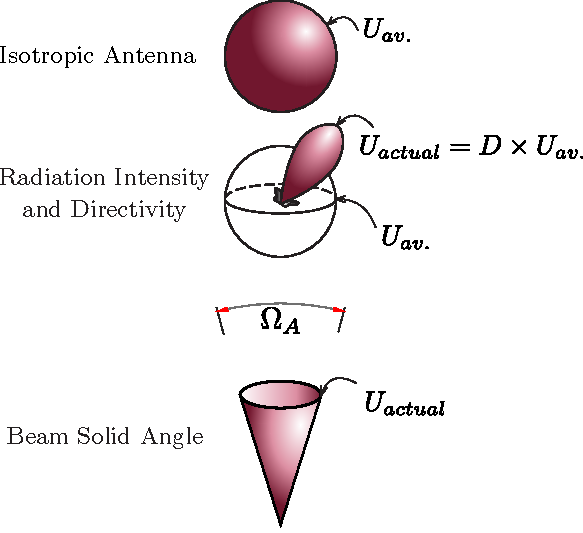
\includegraphics[width=1.20\textwidth]{antenna_dir.pdf}
            \end{figure}
        \end{column}
    \end{columns}
\end{frame}



\begin{frame}
    \frametitle{Finding the Beam Solid Angle}
\small
    Lets first consider a uniformly excited, uniformly spaced linear array where all the elements are \textit{isotropic} ($EF = 1$). From the previous lecture, we have:
    \small
    \begin{align}
        |AF|^2 {}=& \left|\frac{\sin N \psi/2 }{N \sin \psi/2 }\right|^2 \equiv \frac{1}{N} + \frac{1}{N^2} \sum_{m = 1}^{N-1} (N - m) \cos m \psi
        \label{eq:id}
    \end{align}
    \small
    Knowing,
    \small
    \begin{align*}
        \psi {}=& k d \cos \theta + \alpha
        \implies \sin \theta \, \dd \theta = -\frac{1}{k d} \, \dd \psi
    \end{align*}
\small
The beam solid angle $\Omega_A$ then becomes:
\small
\begin{align}
    \Omega_A {}=& \int_{0}^{2 \pi} \dd \phi \int_{0}^{\pi} |AF(\theta)|^2 \dd \theta = 2 \pi \int_{kd + \alpha}^{{-kd + \alpha}} |AF(\psi)|^2 \left(\frac{-1}{kd}\right) \dd \psi \nonumber \\
    {}=& \frac{2 \pi }{k d} \int_{-kd + \alpha}^{{kd + \alpha}} |AF(\psi)|^2 \dd \psi
    \label{eq:omega_A}
\end{align}
\end{frame}


\begin{frame}
    \frametitle{Some Further Computations}

    Solving \eqref{eq:id} and \eqref{eq:omega_A} we get:
    \begin{align*}
        \Omega_{A} &=\frac{2 \pi}{k d}\left[\frac{1}{N} \int_{-k d+\alpha}^{k d+\alpha} \dd \psi+\frac{2}{N^{2}} \sum_{m=1}^{N-1}(N-m) \int_{-k d+\alpha}^{k d+a} \cos m \psi \dd \psi\right] \\
        &=\frac{2 \pi}{k d}\left[\left.\frac{1}{N} \psi\right|_{-k d+\alpha} ^{k d+\alpha}+\left.\frac{2}{N^{2}} \sum_{m=1}^{N-1}(N-m) \frac{\sin m \psi}{m}\right|_{-k d+\alpha} ^{k d+\alpha}\right] \\
        &=\frac{2 \pi}{k d}\left[\frac{1}{N}(2 k d)+\frac{2}{N^{2}} \sum_{m=1}^{N-1} \frac{N-m}{m}[\sin m(k d+\alpha)-\sin m(-k d+\alpha)]\right]
        \end{align*}
    Using the trigonometric identity, $\sin (a+b) = \sin a \, \cos b + \cos a \, \sin b$, we get:
    \begin{tcolorbox}[colback=blue!5]
        \begin{align*}
            \Omega_A   &=\frac{4 \pi}{N}+\frac{4 \pi}{N^{2}} \sum_{m=1}^{N-1} \frac{N-m}{m k d} 2 \cos m \alpha \, \sin m k d
           \end{align*}
  \end{tcolorbox}
\end{frame}

\begin{frame}
    \frametitle{Directivity Expressions}
The directivity for broadside and end-fire arrays is thus:

\begin{align*}
    D {}=& \frac{4\pi }{\Omega_A} = \frac{1}{\frac{1}{N}+\frac{1}{N^{2}} \sum_{m=1}^{N-1} \frac{N-m}{m k d} 2 \cos m \alpha \, \sin m k d}
\end{align*}

For arrays such as the \textit{Hanson-Woodyard} arrays, there is an additional renormalisation factor that accounts for the \textcolor{red}{excess phase delay, $\delta$},

\begin{align}
    D_{\text{General}} {}=&  \frac{\left|\frac{\sin (N \delta/2 )}{N \sin \delta/2 }\right|^2}{\frac{1}{N}+\frac{1}{N^{2}} \sum_{m=1}^{N-1} \frac{N-m}{m k d} 2 \cos m \alpha \, \sin m k d}
    \label{eq:directivity}
\end{align}
\end{frame}

\begin{frame}
    \frametitle{Visualising the Directivity}
In general, the directivity from \eqref{eq:directivity} can be visualised as:
\begin{figure}[h!]
    \centering
    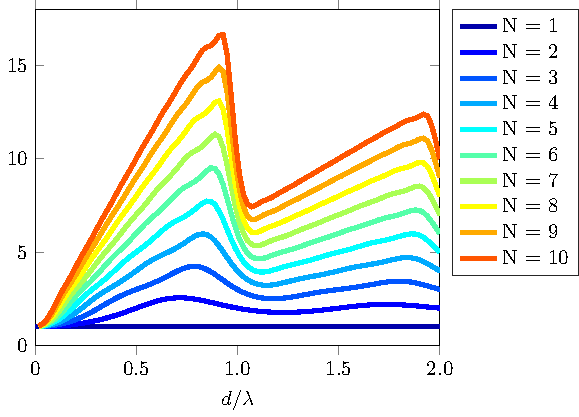
\includegraphics[width=0.75\textwidth]{directivity.pdf}
    \caption{Seeing the directivity as a function of element spacing $d$ and number of elements $N$.}
    \label{fig:directivity}
\end{figure} 
\end{frame}

\section{Multidimensional Arrays}

\begin{frame}
        \frametitle{Planar Arrays}
        \begin{columns}[T]
            \begin{column}{.4\textwidth}
                \begin{outline}
                    \1 So far, the 1D arrays we have looked at only yield beamscanning along one angle $\theta$.
                    \1 Using multidimensional arrays, we can:
                    \2 Obtain pencil beams
                    \2 Higher directivity and gain
                    \2 Maneuver beams in both elevation and azimuthal planes.
                    \1 We can have elliptical or rectangular shapes in the 2D case
                \end{outline}
            \end{column}
            \begin{column}{.6\textwidth}
                \begin{figure}[h!]
                    \centering
                    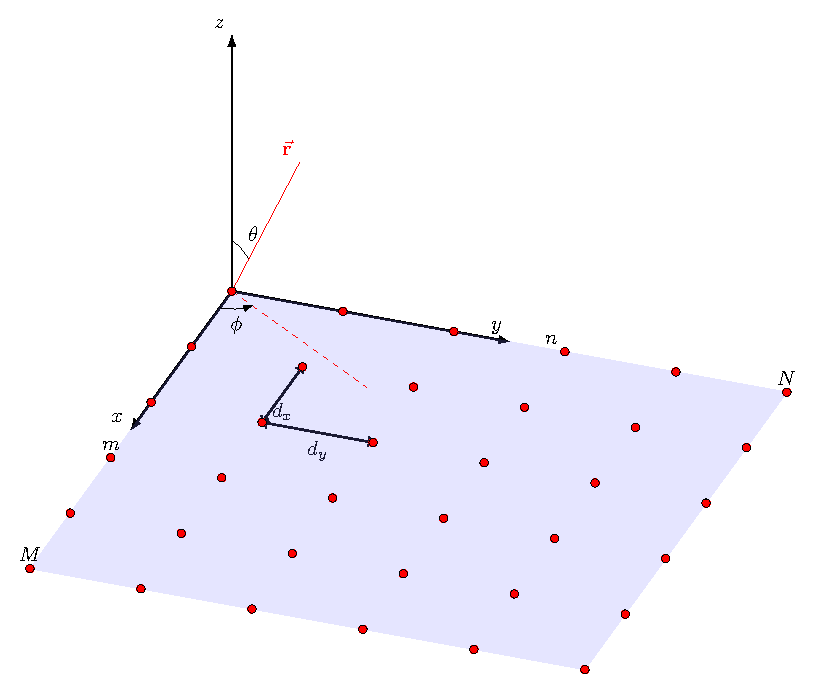
\includegraphics[width=0.95\textwidth]{planar_array.pdf}
                    \caption{A 2D rectangular array.}
                \end{figure}
            \end{column}
        \end{columns}
\end{frame}


\begin{frame}
    \frametitle{Array Factor for Multidimensional Arrays}
    Generally, the Array Factor for an 3D array can be described by first expressing the elements in the form of a position vector:
    \small
    \begin{align*}
        \vu*{r'}_{mn} {}=& \vu{x} \, {d}_{mn} + \vu{y} \, {y'}_{mn} + \vu{z} \, {z'}_{mn}
    \end{align*}
    Then,
    \begin{align*}
        AF (\theta, \phi ) {}=& \sum_{m = 1}^{M} \sum_{n = 1}^{N} I_{mn} \exp(\j (k \, \vu{r}\cdot \, \vu{r'}_{mn} + \alpha_{mn}))
    \end{align*}
    In the normalised form, we can write AF as:
    \begin{align*}
        AF (\theta, \phi) {}=&  \frac{\sin M \psi_x/2 }{{M \sin \psi_x/2}} \, \frac{\sin N \psi_y/2 }{{N \sin \psi_y/2}} \\
        \text{where,} \\
        \psi_x  {}=& k d_x \sin \theta \cos \phi + \alpha_x \, \\
        \psi_y  {}=& k d_y \sin \theta \sin \phi + \alpha_y
    \end{align*}
\end{frame}

\begin{frame}
    \frametitle{Example - 5 x 5 Planar Array}

    Considering a $5 \times 5$ planar array with element spacings $d_x = d_y =  \lambda/2$ and the phases $\alpha_x = \alpha_y = -\pi/(2 \sqrt{2})$. The radiation pattern looks like:
    \begin{figure}[htbp]
        \centering
        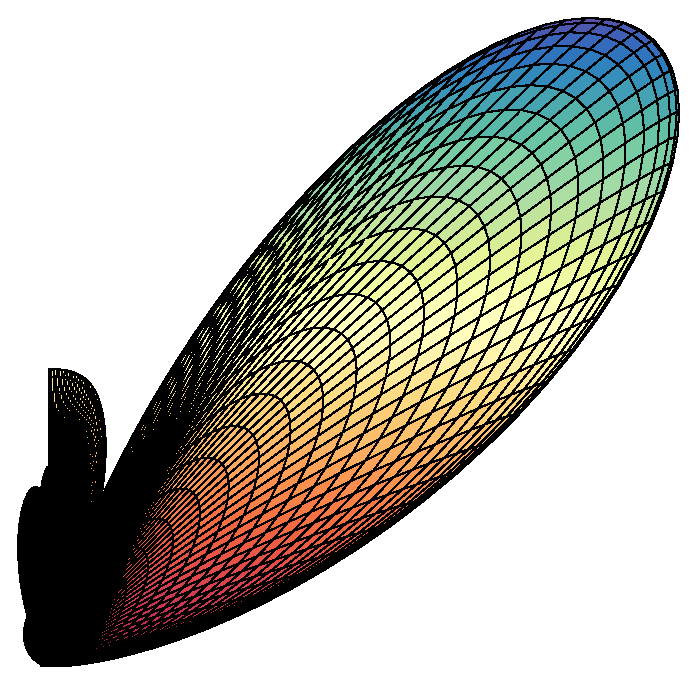
\includegraphics[width=.35\textwidth]{3d_polar_plot_3.eps}
        \caption{Radiation Pattern in the Cartesian coordinates.}
    \end{figure}
\end{frame}

\section{Feeding Networks}


\begin{frame}
    \frametitle{Antenna Array Feeds}
    \begin{columns}[] % align columns
        \begin{column}{.6\textwidth}
            \begin{outline}
                \1 The main benefit of phased array antennas is there is no need for \textit{mechanical motion}.
                \2 Beam can be steered using electronics
                \1 A disadvantage is each antenna element \textit{must} have a transmission path to the receiver
                \2 This is done both via hardware and software
            \end{outline}   
        \end{column}
        \begin{column}{.4\textwidth}
            \begin{figure}[h!]
                \centering
                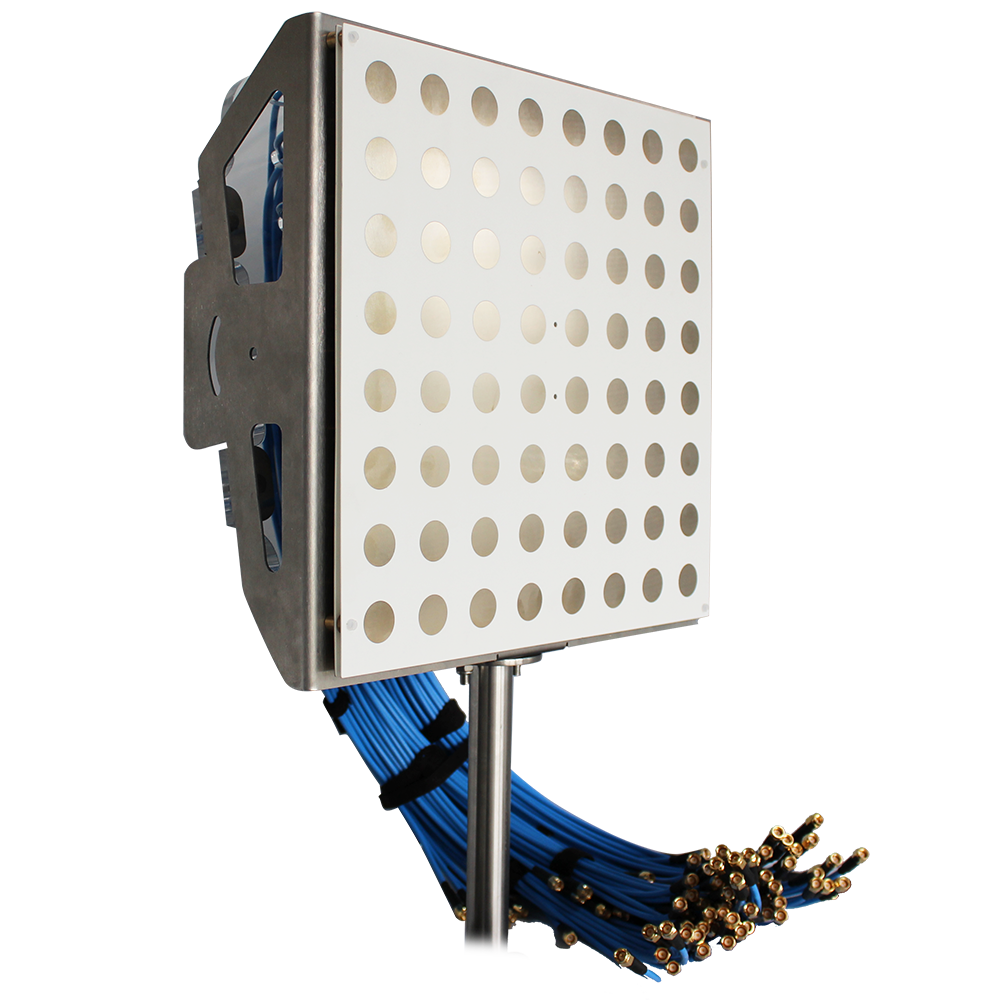
\includegraphics[width=.8\textwidth]{CMM.100.A_01.png}
                \caption{Feeding Cables out of a Massive MIMO Phased Array Antenna}
            \end{figure}

        \end{column}%
    \end{columns}
\end{frame}


\begin{frame}
    \frametitle{Corporate Feeding Network}
    \begin{columns}[] % align columns
        \begin{column}{.5\textwidth}
            \begin{outline}
                \small
                \1 Most common feeding network
                \2 Also called \textit{parallel} feed
                \1 We have equal line lengths to each element
                \2 Phase and amplitude are same across the elements
                \1 Corporate feed can be operated at many frequencies
                \2 We call it wideband as the operation is independent of frequency
            \end{outline}   
        \end{column}
        \begin{column}{.5\textwidth}
            \small
            \begin{figure}[h!]
                \centering
                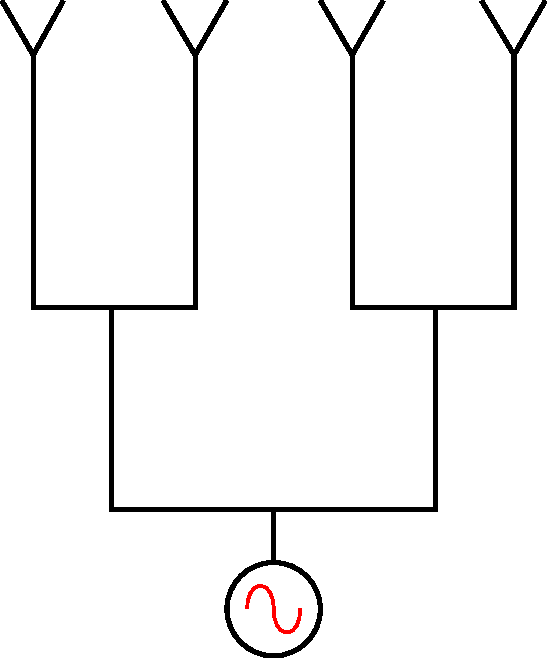
\includegraphics[width=.45\textwidth]{corporate.pdf}
            \end{figure}
            \begin{figure}[h!]
                \centering
                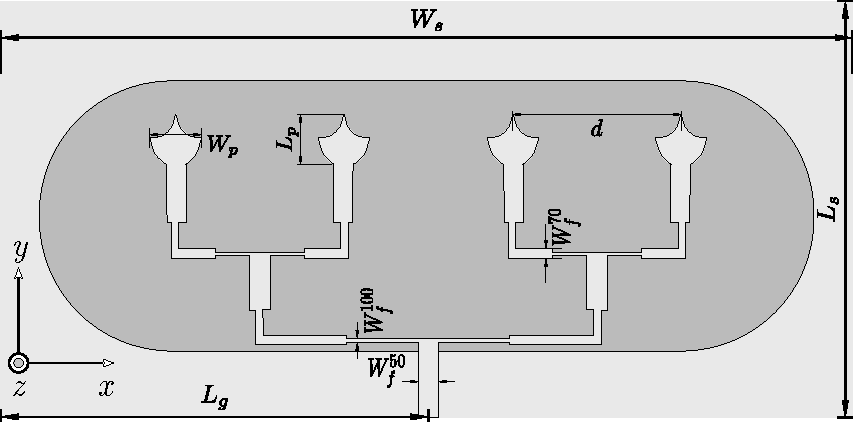
\includegraphics[width=.75\textwidth]{PICA Array.pdf}
                \caption{A Planar Inverted Cone Antenna Array \, \footnotemark[1].}
            \end{figure}
        \end{column}%
    \end{columns}
    \footnotetext[1]{Abdoalbaset al Abohmra et al. “An Ultrawideband Microfabricated Gold-based Antenna Array for Terahertz Communication”. In: IEEE AWPL (2021). ISSN: 1548-5.}
\end{frame}

\begin{frame}
    \frametitle{Series Feeding Network}
    \begin{columns}[] % align columns
        \begin{column}{.6\textwidth}
            \begin{outline}
                \1 Simplest feeding architecture
                \2 Phase difference can be easily generated
                \1 However, practically loss occurs along the series line
                \2 This results in unequal amplitudes across the elements
                \1 By changing the frequency, the electrical line length of the feed is changed.
                \2 Due to this, we have dispersion that limits bandwidth
            \end{outline}   
        \end{column}
        \begin{column}{.4\textwidth}
            \begin{figure}[h!]
                \centering
                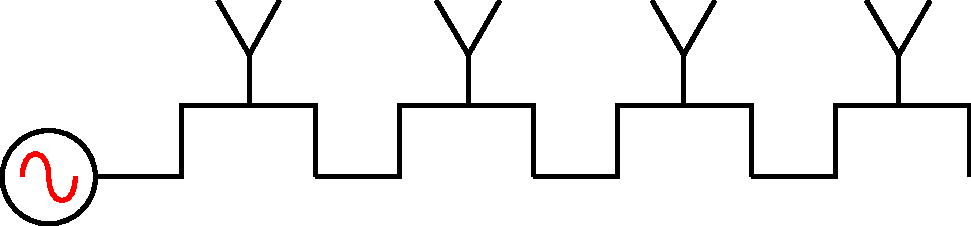
\includegraphics[width=.8\textwidth]{series.pdf}
                \caption{A series feeding network}
            \end{figure}
        \end{column}%
    \end{columns}
\end{frame}

\begin{frame}
    \frametitle{The Hybrid Feeding Network}
    \begin{columns}[] % align columns
        \begin{column}{.5\textwidth}
            \begin{outline}
                \1 Suitable for very large arrays
                \2 Additional phase shift is introduced commonly through diodes (PIN etc.)
                \1 MEMS based switches can turn a particular arm on or off.
                \2 Such feeds can withstand high power inputs
                \1 By changing the frequency, the electrical line length of the feed is changed.
                \2 Due to this, we have dispersion that limits bandwidth
            \end{outline}   
        \end{column}
        \begin{column}{.5\textwidth}
            \begin{figure}[h!]
                \centering
                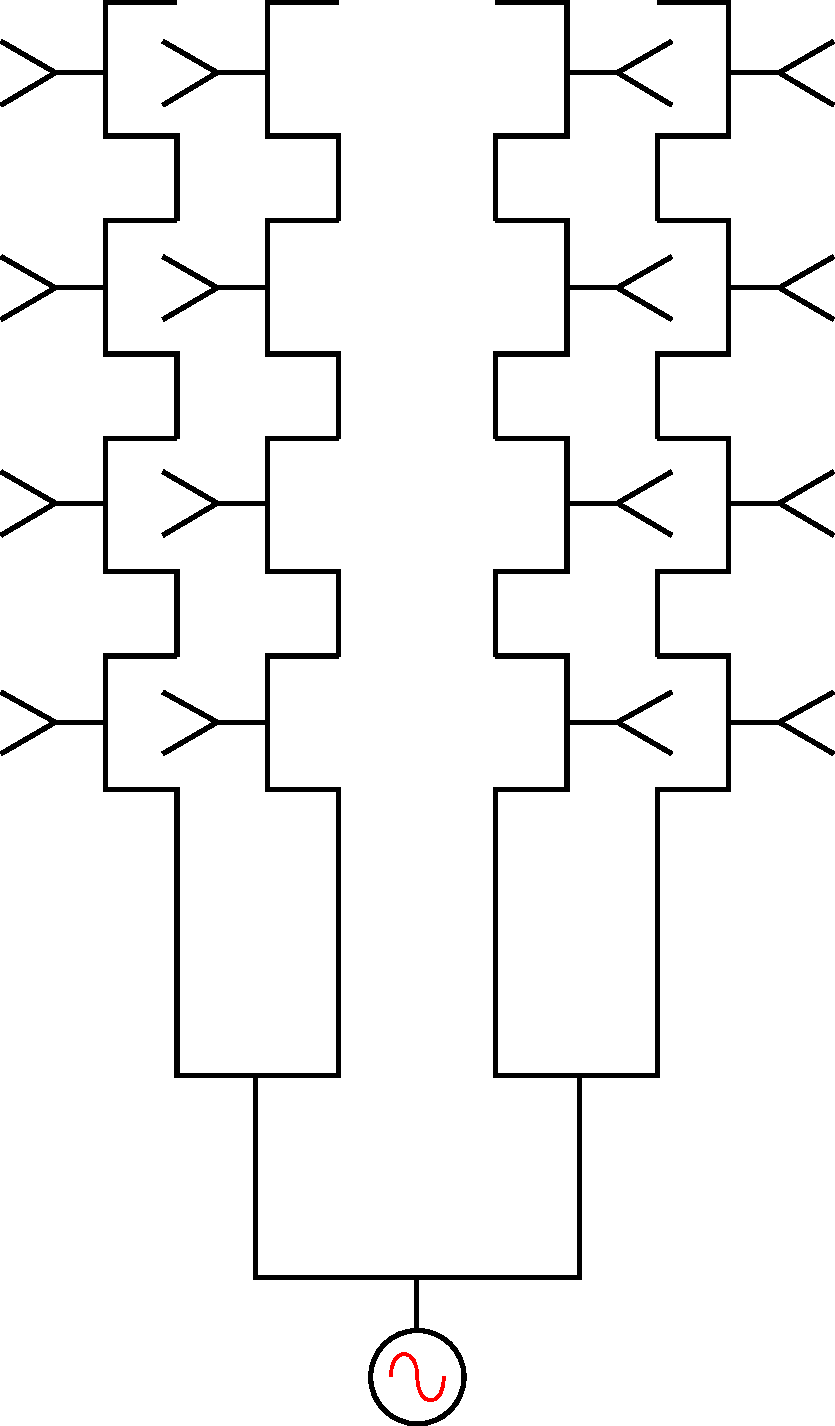
\includegraphics[width=.6\textwidth]{hybrid.pdf}
                \caption{A hybrid corporate-series feeding network}
            \end{figure}
        \end{column}%
    \end{columns}
\end{frame}

\begin{frame}
    \frametitle{Other Feeding Networks}
    \begin{columns}[] % align columns
        \begin{column}{.7\textwidth}
            \begin{outline}
                \small
                \1 For millimetre wave communications, corporate and series feeding architectures become very complicated
                \1 Other techniques such as \textit{sequentially rotated phase} feeding networks are emerging as attractive candidates
                \2 Each antenna element is physically rotated
                \2 Additionally, there is a phase shift to each element
                \1 The advantage over corporate feeding network is that the \textit{resonant} response can be obtained at a higher range of frequencies
                \2 Ensures radiation pattern integrity
            \end{outline}   
        \end{column}
        \begin{column}{.4\textwidth}
            \begin{figure}[h!]
                \centering
                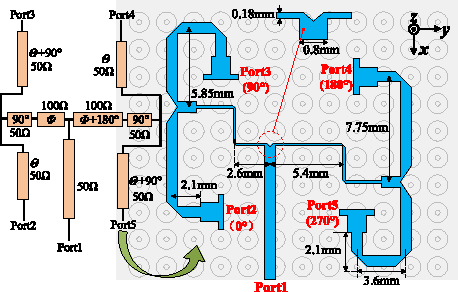
\includegraphics[width=.95\textwidth]{SRP.pdf}
                \caption{\small A sequentially rotated phase feeding network \footnotemark[1].}
            \end{figure}
        \end{column}%
    \end{columns}
    \footnotetext[1]{Chaojun Ma, Zu-Hui Ma, and Xiupu Zhang. “Millimeter-Wave Circularly Polarized Array Antenna Using Substrate-Integrated Gap Waveguide Sequentially Rotating Phase Feed", In: IEEE AWPL (2019). ISSN: 1548-5757.}
\end{frame}

\section{Software Defined Radio}

\begin{frame}
    \frametitle{Software Defined Radio - Motivation}
    \begin{outline}
    \1 A communication system consists of many layers of operations.
    \1 The physical layer is the most important of all.
    \1 Typically, physical layer processing is done via dedicated hardware
    \1 Radio is the technology through which signals are wirelessly transmitted and received
    \1 Software-defined radio has some or all physical layer functions implemented via hardware
\end{outline}
\end{frame}

\begin{frame}
    \frametitle{Software Defined Radio}
\begin{figure}[h!]
    \centering
    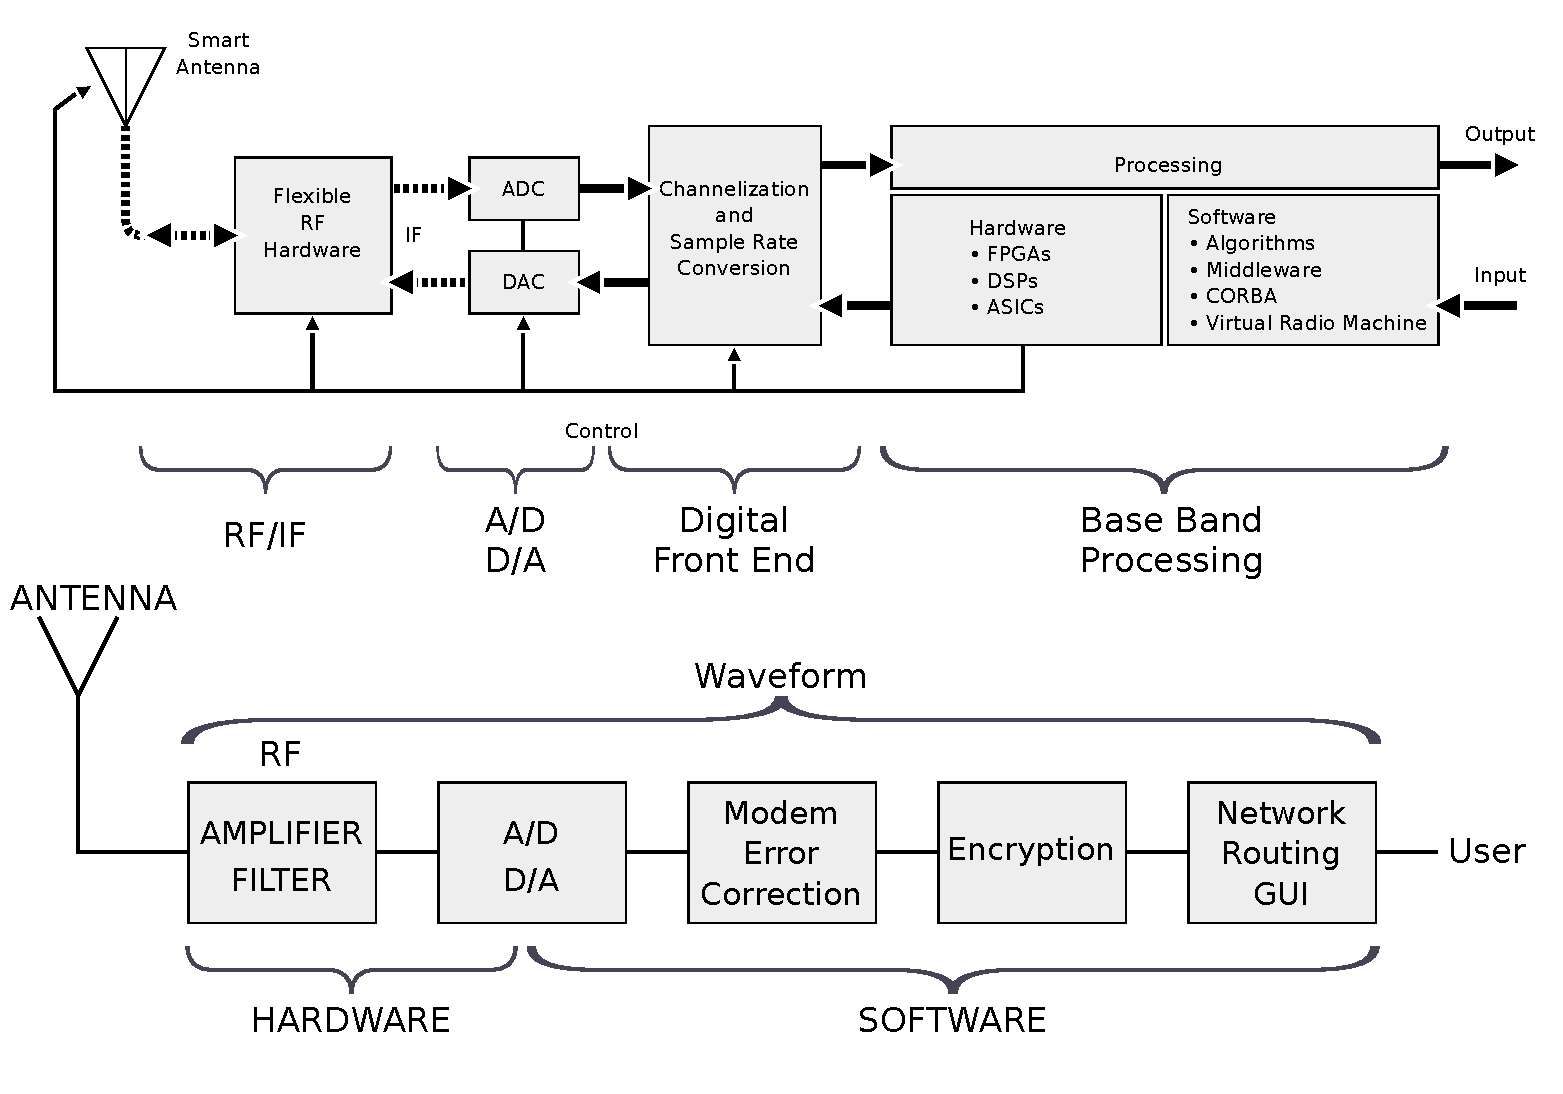
\includegraphics[width=.8\textwidth]{SDR_et_WF.pdf}
    \caption{A Typical SDR workflow}
\end{figure}
\end{frame}

\begin{frame}
    \frametitle{GNU Radio}
    \begin{columns}[] % align columns
        \begin{column}{.5\textwidth}
        \begin{outline}
            \small
    \1 A graphical user interface consisting of \textit{flowgraphs} through which different signal processing functions such as analog-digital conversion can be performed.
    \1 Some additions let us write \texttt{Python} codes within each block
    \1 The software is meant to interface with Universal Software Radio Peripheral (USRP) modules to construct a complete communication system.
\end{outline}   
\end{column}
\begin{column}{.5\textwidth}
\begin{figure}[h!]
    \centering
    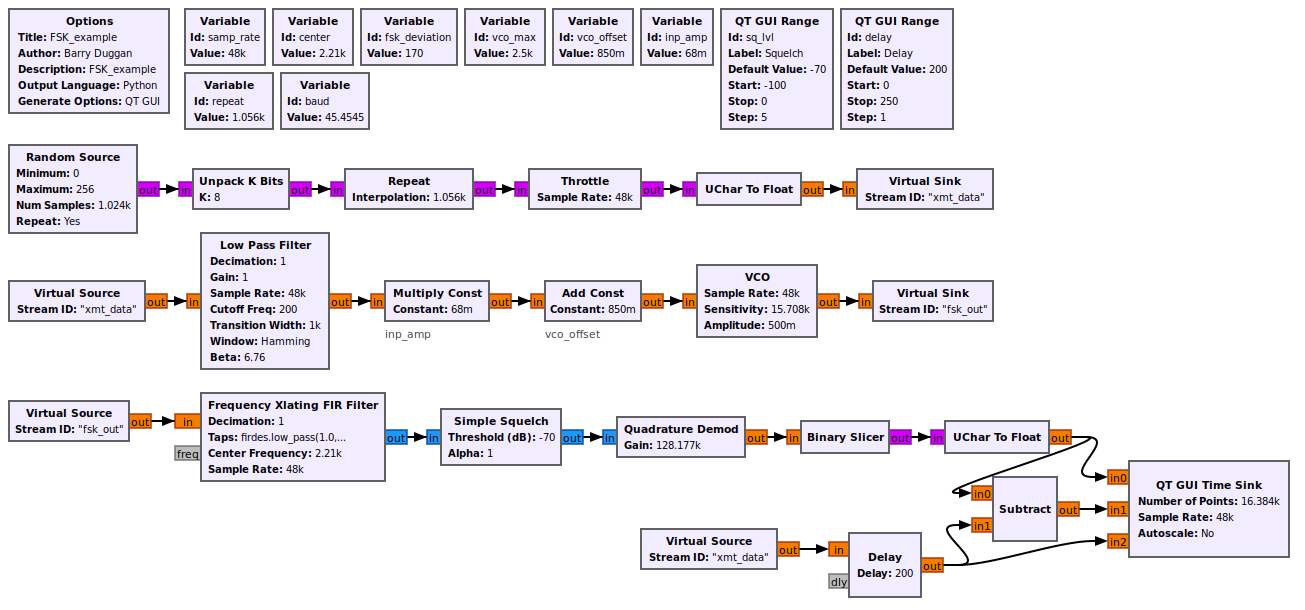
\includegraphics[width=.95\textwidth]{FSK_example_fg.png}
    \caption{GNU Radio Interface.}
\end{figure}
\end{column}%
\end{columns}   

\end{frame}
\end{document}
